\section{Results}
\label{sec:results}

All results in this section come from the single specification set out in Section~3.
No parameter was selected by reference to the evaluation period, and every
specification examined is reported, including those that are unfavourable to the
framework.

\subsection{Headline Performance}

Table~\ref{tab:main} reports the primary comparison over the 4{,}689 trading sessions from
7~January 2008 to 26~August 2026.

\begin{table}[!ht]
\centering
\caption{Primary results, ten-asset universe, January 2008 to August 2026. Sharpe
ratios use a zero risk-free rate and are computed as compound annual growth divided by
annualised volatility. Benchmarks are rebalanced daily and charged no transaction costs.}
\label{tab:main}
\small
\begin{tabular}{p{4.4cm}rrrrr}
\hline
& \textbf{CAGR} & \textbf{Volatility} & \textbf{Sharpe} & \textbf{Max DD} & \textbf{Calmar} \\
\hline
Regime-conditional strategy & 5.65\% & 6.44\% & 0.878 & $-18.98$\% & 0.298 \\
Equal-weight benchmark & 8.45\% & 13.45\% & 0.628 & $-36.08$\% & 0.234 \\
Inverse-volatility benchmark & 7.46\% & 8.78\% & 0.849 & $-24.09$\% & 0.309 \\
Equal-weight at strategy volatility & 4.19\% & 6.44\% & 0.651 & $-18.69$\% & 0.224 \\
\hline
\end{tabular}
\end{table}

Three readings of Table~\ref{tab:main} are warranted, and they do not all favour the framework.

Against the equal-weighted benchmark the framework improves the Sharpe ratio from 0.628
to 0.878, a gain of 40 per cent, and reduces maximum drawdown from $-36.08$ per cent to
$-18.98$ per cent, a reduction of 47 per cent. It does so while earning a lower
compound return, 5.65 per cent against 8.45 per cent per annum. The framework is not a
return-enhancing strategy and is not presented as one; it is a risk-reduction strategy
whose return sacrifice is smaller than its risk reduction.

Against the volatility-matched equal-weighted benchmark, which removes the mechanical
advantage a lower-risk portfolio enjoys in any ratio comparison, the framework retains
a Sharpe advantage of 0.878 against 0.651, but loses on maximum drawdown, $-18.98$ per
cent against $-18.69$ per cent. Deleveraging a diversified benchmark is therefore a
competitive way to reduce worst-case loss, and the framework's drawdown advantage over
the unlevered benchmark should not be read as evidence that it dominates every
risk-reduced alternative.

Against the inverse-volatility benchmark the comparison is mixed. The framework holds a
higher Sharpe ratio, 0.878 against 0.849, and a materially smaller maximum drawdown,
$-18.98$ per cent against $-24.09$ per cent, but a lower Calmar ratio, 0.298 against
0.309, because inverse-volatility weighting compounds faster. Elementary risk weighting
remains a strong comparator on a diversified multi-asset universe, and the margin over
it is narrow enough that it should be read as a tie on risk-adjusted return rather than
as a win.

Figure~2 shows the cumulative growth of one unit of capital and Figure~3 the drawdown
profile of each series.

\begin{figure*}[t]
\centering
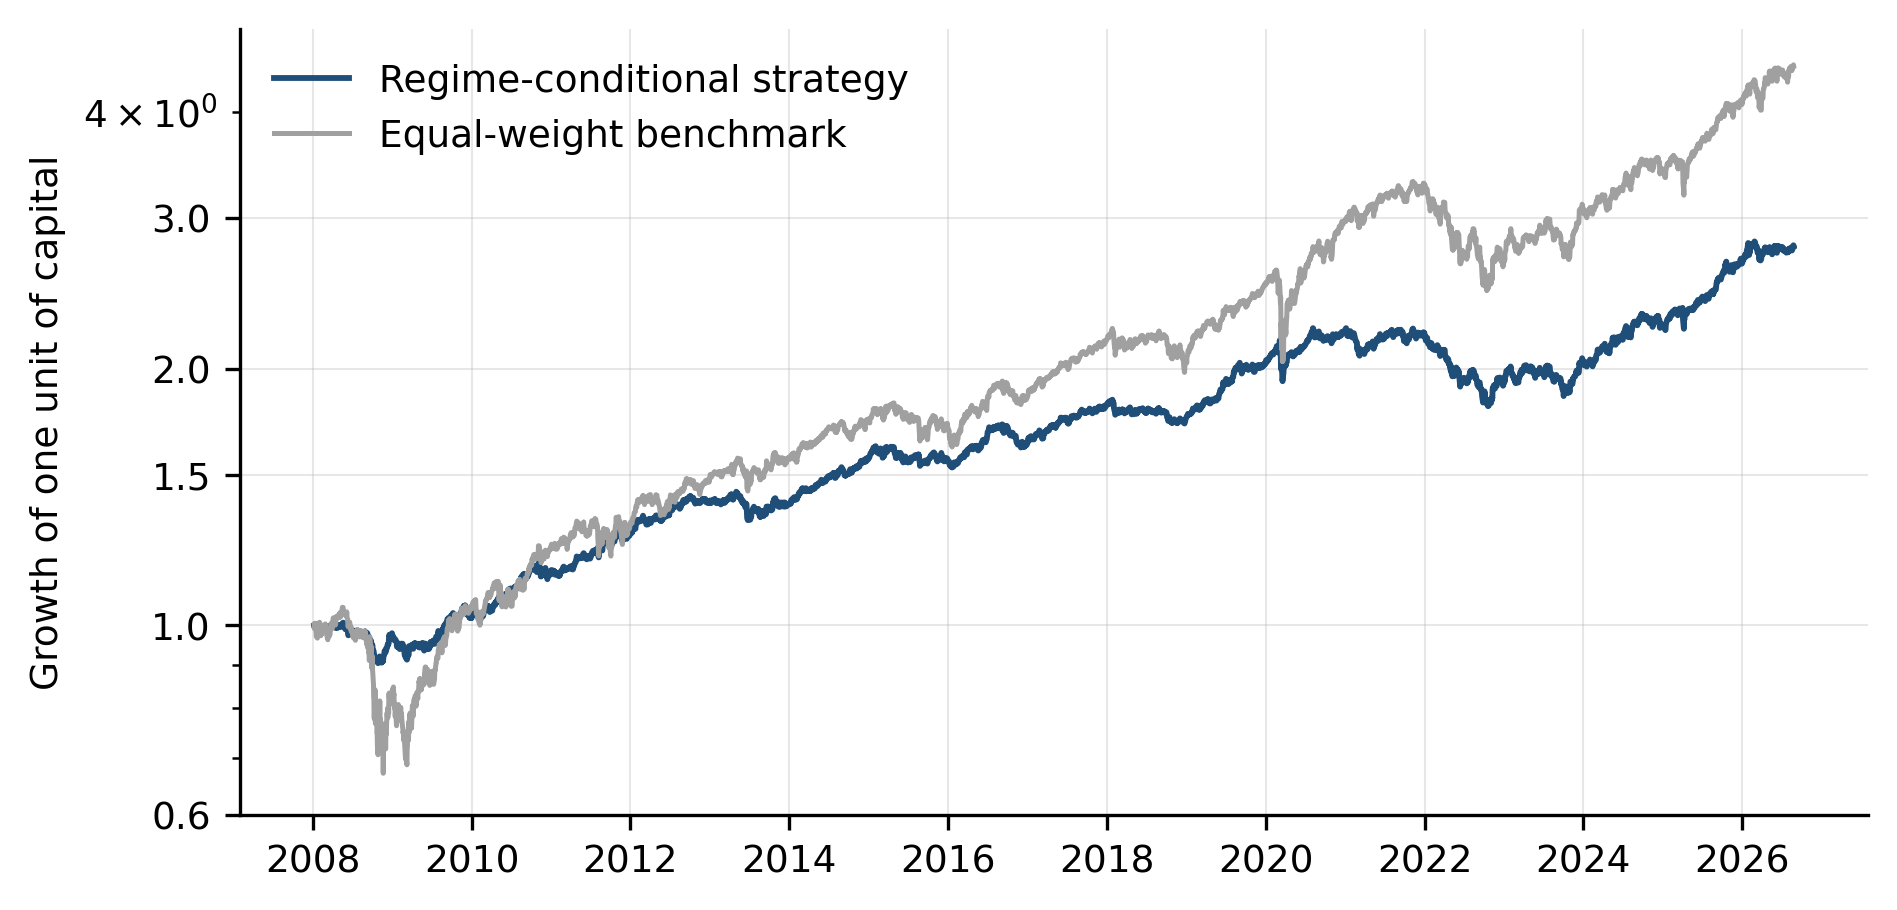
\includegraphics[width=\textwidth]{single column/images/fig_cumret.png}
\caption{Cumulative growth of one unit of capital, logarithmic scale}
\label{fig:cumret}
\end{figure*}

\begin{figure*}[t]
\centering
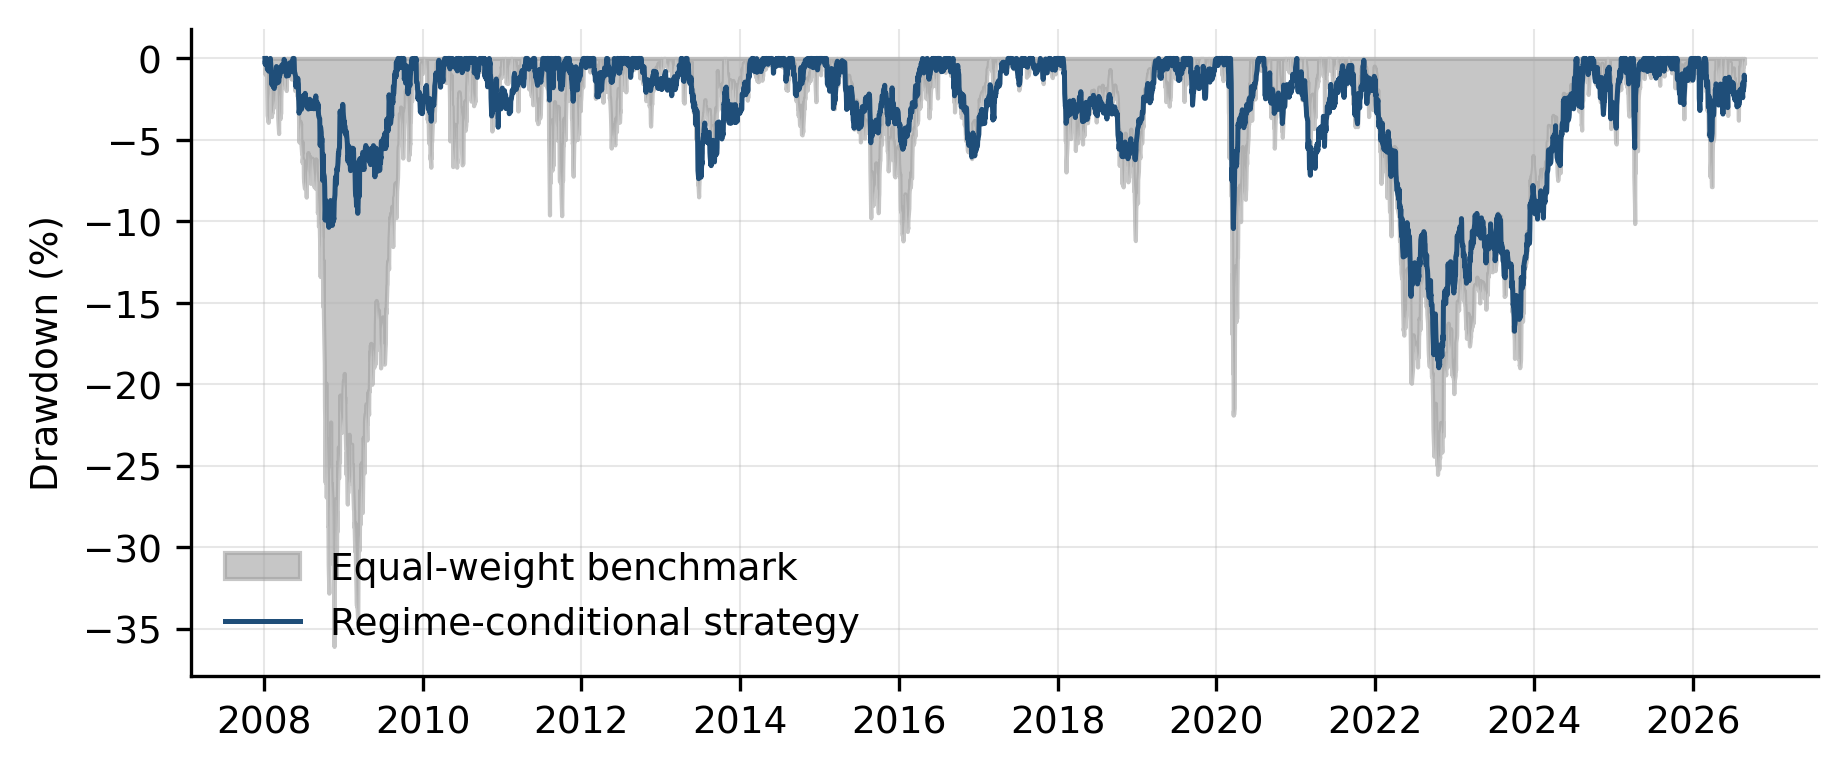
\includegraphics[width=\textwidth]{single column/images/fig_drawdown.png}
\caption{Drawdown from running peak}
\label{fig:drawdown}
\end{figure*}

The two figures make the shape of the result visible. The framework's equity curve
tracks below the benchmark through extended advances---most conspicuously 2013, 2017,
2021 and 2023---and separates upward during 2008, 2011, 2020 and 2022. The drawdown
plot shows the same asymmetry more directly: the benchmark reaches $-36$ per cent in
2008 and $-25$ per cent in 2022, while the framework's deepest excursions are
approximately half as large. Recovery is correspondingly faster, since a shallower loss
requires a smaller subsequent gain to restore the previous peak.

\subsection{Out-of-Sample Holdout, 2024--2026}
\label{sec:holdout}

Every specification decision in this study---the universe, the feature set, the number of
regimes, the risk budget, the rebalancing interval and the cost assumption---was fixed
before any session after December~2023 was examined. The 665 sessions from January~2024
to August~2026 therefore function as a holdout rather than as a further robustness check
on the same data. Table~\ref{tab:holdout} reports both blocks side by side.

\begin{table}[!ht]
\centering
\caption{Performance before and after the holdout boundary. The two blocks are disjoint;
the full-sample results of Table~\ref{tab:main} pool them.}
\label{tab:holdout}
\small
\begin{tabular}{p{4.9cm}rrrr}
\hline
& \multicolumn{2}{c}{\textbf{2008--2023} ($n=4{,}024$)} & \multicolumn{2}{c}{\textbf{2024--2026} ($n=665$)} \\
& \textbf{Sharpe} & \textbf{Max DD} & \textbf{Sharpe} & \textbf{Max DD} \\
\hline
Regime-conditional strategy & 0.738 & $-18.98$\% & 1.614 & $-5.48$\% \\
Equal-weight benchmark & 0.532 & $-36.08$\% & 1.391 & $-10.13$\% \\
Inverse-volatility benchmark & 0.764 & $-24.09$\% & 1.397 & $-6.70$\% \\
Equal-weight at strategy volatility & 0.560 & $-17.66$\% & 1.378 & $-7.04$\% \\
No regime timing, full exposure & 0.785 & $-22.53$\% & 1.710 & $-6.47$\% \\
\hline
\end{tabular}
\end{table}

In the holdout the framework records a higher Sharpe ratio than all three benchmarks,
1.614 against 1.391, 1.397 and 1.378, and a smaller maximum drawdown than all three,
$-5.48$ per cent against $-10.13$, $-6.70$ and $-7.04$ per cent. Two of those comparisons
reverse the in-sample ordering: the inverse-volatility benchmark and the
volatility-matched equal-weighted benchmark both beat the framework on Sharpe ratio
before 2024 and both trail it afterwards. The deepest equal-weighted drawdown in the
holdout, the 34-session decline from 20~February to 8~April~2025, returned $-10.05$\% for
the benchmark against $-4.63$\% for the framework, an advantage of 5.42 percentage points
that is consistent with the four earlier episodes in Table~\ref{tab:episodes}.

Three qualifications limit what this establishes. First, 665 sessions are too few to
settle anything on their own: the bootstrap interval for the Sharpe difference in the
holdout is $[-0.352, 0.742]$, wider than the full-sample interval and comfortably
containing zero, and the framework again earns less in absolute terms, giving up 3.07
percentage points of annual return ($p = 0.348$). Second, the holdout contains no
episode comparable to 2008 or 2020; every series in it posts a Sharpe ratio above 1.3,
so the period is benign and the relevant information is the ordering rather than the
level. Third, the ablation ordering is unchanged---the variant with no regime timing at
full exposure again records the highest Sharpe ratio, 1.710---so the holdout does not
rescue any claim that Section~\ref{sec:ablation} rejects.

What the holdout does establish is narrower and still worth stating. The framework's
defensive behaviour is not an artefact of the sample on which it was specified. It was
built without reference to these sessions, and on them it continues to reduce drawdown
against every benchmark considered while remaining competitive on risk-adjusted return.

\subsection{Robustness Across Specifications}
\label{sec:robust}

The primary configuration fixes a random seed, a covariance estimation window and a
rebalancing interval. Table~\ref{tab:sweep} reports every combination of three seeds, two estimation
windows and three rebalancing intervals, so that the reported result can be located
within the distribution of specifications rather than presented in isolation.

\begin{table}[!ht]
\centering
\caption{Specification sweep. All eighteen cells reported; the last two columns record
whether the cell beats the equal-weight benchmark on each measure. Sharpe ratios here are
the annualised arithmetic mean over volatility, so that all eighteen cells are computed
identically; on the same basis the equal-weight benchmark attains 0.670 with a maximum
drawdown of $-36.1$\%.}
\label{tab:sweep}
\small
\begin{tabular}{rrrrrcc}
\hline
\textbf{Seed} & \textbf{Cov. window} & \textbf{Rebalance} & \textbf{Sharpe} & \textbf{Max DD} & \textbf{Sharpe win} & \textbf{DD win} \\
\hline
0 & 126 & 10 & 0.868 & $-20.7$\% & yes & yes \\
0 & 126 & 21 & 0.954 & $-19.6$\% & yes & yes \\
0 & 126 & 42 & 0.924 & $-19.7$\% & yes & yes \\
0 & 252 & 10 & 0.823 & $-20.8$\% & yes & yes \\
0 & 252 & 21 & 0.905 & $-19.0$\% & yes & yes \\
0 & 252 & 42 & 0.899 & $-20.4$\% & yes & yes \\
7 & 126 & 10 & 0.881 & $-20.6$\% & yes & yes \\
7 & 126 & 21 & 0.956 & $-19.6$\% & yes & yes \\
7 & 126 & 42 & 0.912 & $-19.6$\% & yes & yes \\
7 & 252 & 10 & 0.818 & $-21.1$\% & yes & yes \\
7 & 252 & 21 & 0.891 & $-19.0$\% & yes & yes \\
7 & 252 & 42 & 0.888 & $-20.4$\% & yes & yes \\
42 & 126 & 10 & 0.853 & $-20.6$\% & yes & yes \\
42 & 126 & 21 & 0.928 & $-19.6$\% & yes & yes \\
42 & 126 & 42 & 0.893 & $-19.7$\% & yes & yes \\
42 & 252 & 10 & 0.813 & $-21.1$\% & yes & yes \\
42 & 252 & 21 & 0.887 & $-19.0$\% & yes & yes \\
42 & 252 & 42 & 0.853 & $-20.4$\% & yes & yes \\
\hline
\end{tabular}
\end{table}

Every one of the eighteen specifications beats the equal-weighted benchmark on both the
Sharpe ratio and maximum drawdown. The Sharpe ratio ranges from 0.813 to 0.956 and the
maximum drawdown from $-21.1$ to $-19.0$ per cent. The primary configuration appears in
this table at 0.887, which is the median of the eighteen values: it is not the best cell,
and the best cell exceeds it by 0.069. Sensitivity to the random seed is small, which
indicates that the mixture fit is stable; sensitivity to the rebalancing interval is
larger, with ten-session rebalancing consistently weakest because it incurs more turnover
for no additional information.

The same sweep is unfavourable on one comparison. In none of the eighteen cells does
the framework beat the volatility-matched equal-weighted benchmark on maximum drawdown.
This is a consistent finding rather than an artefact of the primary configuration, and
it bounds the drawdown claim precisely: the framework reduces drawdown relative to an
unlevered diversified benchmark, not relative to every portfolio held at the same
volatility.

\subsection{Behaviour in Stress Episodes}

Table~\ref{tab:episodes} reports cumulative returns over four episodes chosen before the analysis on the
basis of documented market history rather than by inspection of the results.

\begin{table}[!ht]
\centering
\caption{Cumulative return over stress episodes. Differences are stated in percentage
points (pp).}
\label{tab:episodes}
\small
\begin{tabular}{p{3.6cm}rrrr}
\hline
\textbf{Episode} & \textbf{Sessions} & \textbf{Strategy} & \textbf{Equal-weight} & \textbf{Difference} \\
\hline
Global financial crisis, Sep 2008--Mar 2009 & 130 & $-7.05$\% & $-29.78$\% & $+22.74$ pp \\
Euro area crisis, Jul--Oct 2011 & 65 & $+3.41$\% & $-7.24$\% & $+10.65$ pp \\
COVID-19 crash, Feb--Mar 2020 & 24 & $-6.29$\% & $-21.28$\% & $+14.99$ pp \\
Inflation bear market, Jan--Oct 2022 & 196 & $-16.76$\% & $-24.49$\% & $+7.73$ pp \\
\hline
\end{tabular}
\end{table}

The framework outperforms in all four episodes, by between 7.7 and 22.7 percentage
points. All four predate the holdout boundary; the deepest benchmark decline after it,
analysed in Section~\ref{sec:holdout}, produced an advantage of 5.4 percentage points. The mechanism is visible in the exposure series: the mixture model classifies
these periods into the transitional or stress state, and the risk budget reduces
invested exposure accordingly. The margin is widest in 2008, the longest and deepest of
the four, and narrowest in 2022, which is consistent with the design---a gradual,
correlated decline across both equities and bonds offers less scope for a de-risking
rule than an abrupt volatility shock does.

Complementing the episode analysis, the framework's average return on the worst
5~per~cent of benchmark sessions ($n = 234$) is $-0.59$ per cent against $-2.01$ per
cent for the benchmark, a cushion of 1.42 percentage points per session. Downside
capture is 0.38 and upside capture 0.41, giving a capture ratio of 0.93. The ratio
being close to unity is informative: the framework participates less in both directions
in roughly equal proportion, so its advantage comes predominantly from carrying less
risk in adverse states rather than from any directional skill.

\subsection{Year-by-Year Performance}

Table~\ref{tab:years} reports every calendar year in the sample, with both wins and losses shown.

\begin{table}[!ht]
\centering
\caption{Calendar year performance. Sharpe and maximum drawdown computed within each
year. 2026 covers January to August only; the sample ends on 26~August 2026.}
\label{tab:years}
\small
\begin{tabular}{rrrrrcc}
\hline
\textbf{Year} & \textbf{Strategy} & \textbf{Equal-weight} & \textbf{Strat. Sharpe} & \textbf{EW Sharpe} & \textbf{Sharpe win} & \textbf{DD win} \\
\hline
2008 & $-2.28$\% & $-16.32$\% & $-0.33$ & $-0.47$ & yes & yes \\
2009 & $+4.36$\% & $+24.91$\% & $0.60$ & $1.18$ & no & yes \\
2010 & $+13.75$\% & $+18.31$\% & $2.05$ & $1.40$ & yes & yes \\
2011 & $+10.36$\% & $+5.75$\% & $1.73$ & $0.45$ & yes & yes \\
2012 & $+8.91$\% & $+13.49$\% & $1.96$ & $1.58$ & yes & yes \\
2013 & $-0.58$\% & $+6.17$\% & $-0.06$ & $0.72$ & no & yes \\
2014 & $+13.03$\% & $+9.97$\% & $2.94$ & $1.49$ & yes & yes \\
2015 & $-0.48$\% & $-1.56$\% & $-0.05$ & $-0.13$ & yes & yes \\
2016 & $+4.85$\% & $+8.49$\% & $0.94$ & $0.97$ & no & yes \\
2017 & $+10.92$\% & $+16.59$\% & $2.65$ & $3.15$ & no & yes \\
2018 & $-3.51$\% & $-5.26$\% & $-0.78$ & $-0.52$ & no & yes \\
2019 & $+15.72$\% & $+22.55$\% & $2.84$ & $3.02$ & no & yes \\
2020 & $+9.63$\% & $+19.32$\% & $1.23$ & $0.96$ & yes & yes \\
2021 & $-0.78$\% & $+10.15$\% & $-0.08$ & $1.12$ & no & no \\
2022 & $-12.99$\% & $-19.30$\% & $-1.55$ & $-1.23$ & no & yes \\
2023 & $+6.83$\% & $+16.53$\% & $0.90$ & $1.52$ & no & yes \\
2024 & $+9.38$\% & $+9.58$\% & $1.25$ & $1.00$ & yes & yes \\
2025 & $+18.53$\% & $+20.17$\% & $2.24$ & $1.67$ & yes & yes \\
2026 & $+4.80$\% & $+10.93$\% & $0.96$ & $1.34$ & no & yes \\
\hline
\end{tabular}
\end{table}

The framework wins on Sharpe ratio in 9 of 19 years and on drawdown in 18 of 19. This
distribution is the honest summary of the strategy: it loses on risk-adjusted return in
most individual years, particularly strong advancing years such as 2009, 2017, 2021 and
2023, and recovers the deficit in the minority of years when the benchmark suffers. The
three years after the holdout boundary follow the same pattern: drawdown wins in all
three, Sharpe wins in two. Two
years merit comment. In 2021 the framework loses on both measures, the only such year,
because the mixture model spent much of that year in the transitional state during what
turned out to be a sustained advance. In 2018 the framework loses on Sharpe despite a
smaller loss in absolute terms, an arithmetic consequence of a smaller negative return
divided by a much smaller volatility.

Figure~4 shows the rolling one-year Sharpe ratio of both series. The framework's rolling
Sharpe is positive in 81.9 per cent of windows against 85.8 per cent for the benchmark,
and exceeds the benchmark in 53.4 per cent of windows. Its advantage is therefore
episodic rather than persistent, which is what Table~\ref{tab:years} leads one to expect.

\begin{figure*}[t]
\centering
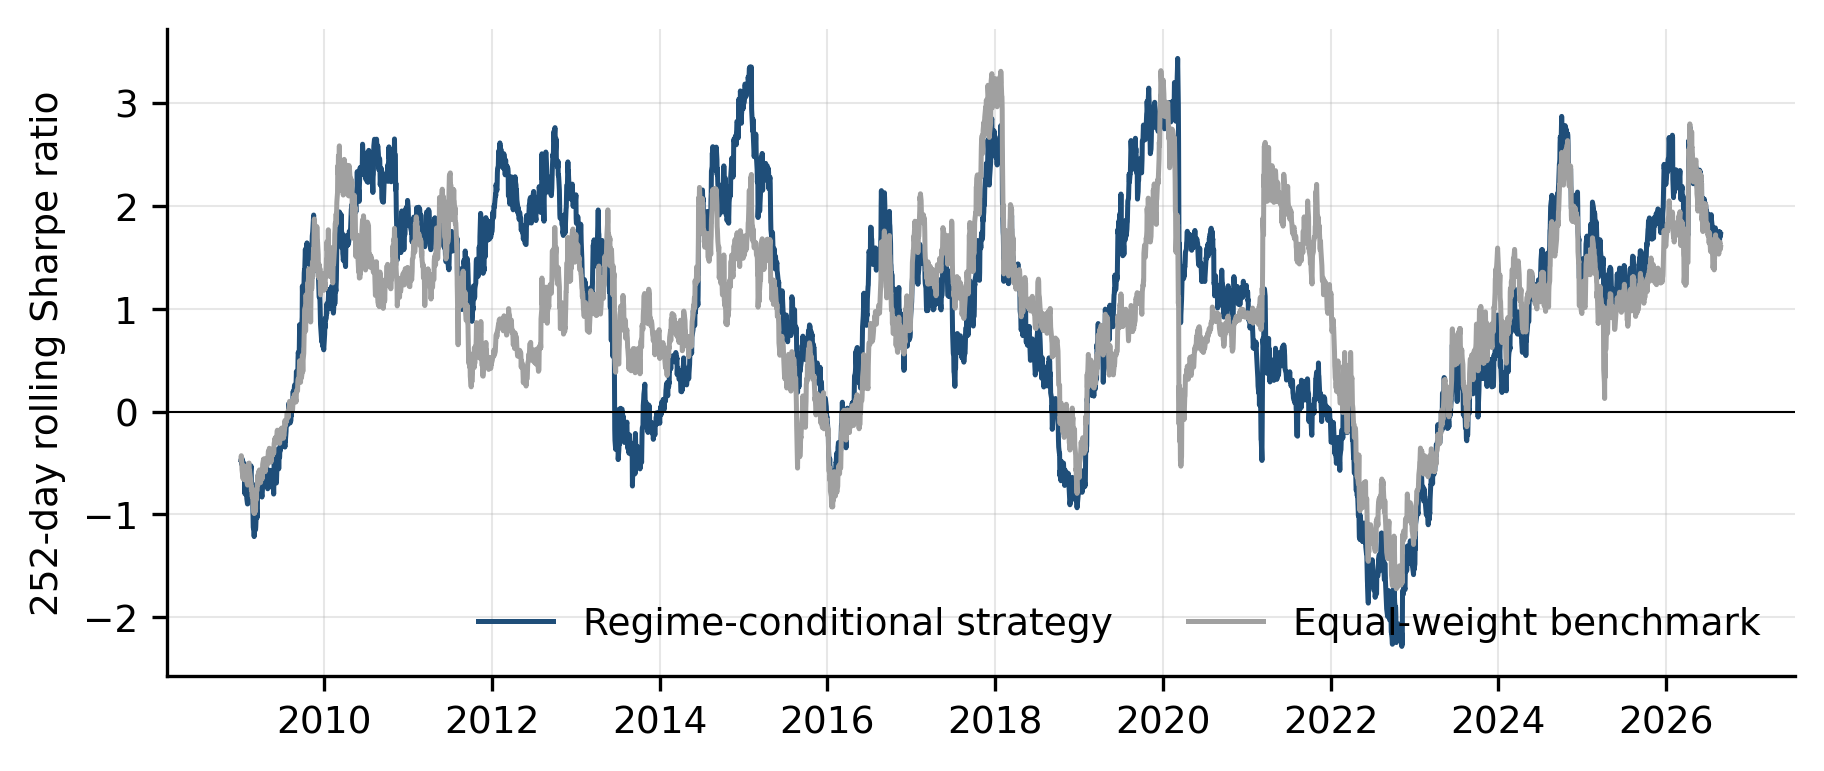
\includegraphics[width=\textwidth]{single column/images/fig_rollsharpe.png}
\caption{Rolling 252-session Sharpe ratio}
\label{fig:rollsharpe}
\end{figure*}

\subsection{Component Ablation}
\label{sec:ablation}

The framework has two active layers, signal fusion and the regime risk budget.
Table~\ref{tab:ablation} removes each in turn. The comparison requires care, because scaling a portfolio
toward cash changes its return and its volatility together; comparing a de-risked
strategy against a fully invested variant therefore confounds the timing of risk with
its level. The first ablation holds average invested exposure fixed at the framework's
own 92.1 per cent and applies it constantly, so that only the timing differs.

\begin{table}[!ht]
\centering
\caption{Component ablation. The matched-exposure control holds the same average
invested exposure as the full framework but applies it without regard to the regime.}
\label{tab:ablation}
\small
\begin{tabular}{p{4.8cm}rrrrr}
\hline
\textbf{Configuration} & \textbf{CAGR} & \textbf{Sharpe} & \textbf{Max DD} & \textbf{Exposure} & \textbf{$p$} \\
\hline
Full framework & 5.65\% & 0.878 & $-18.98$\% & 92.1\% & --- \\
No regime timing, same average exposure & 5.43\% & 0.795 & $-22.26$\% & 92.1\% & 0.695 \\
No regime timing, full exposure & 6.91\% & 0.923 & $-22.53$\% & 100.0\% & 0.016 \\
No signal layer & 5.75\% & 0.908 & $-18.87$\% & 92.1\% & 0.650 \\
Equal-weight benchmark & 8.45\% & 0.628 & $-36.08$\% & 100.0\% & --- \\
\hline
\end{tabular}
\end{table}

The first comparison is the one the framework is built on, and it succeeds. Holding
average exposure fixed, allocating that exposure according to the regime rather than
uniformly raises the Sharpe ratio from 0.795 to 0.878 and improves maximum drawdown
from $-22.26$ to $-18.98$ per cent. The difference in mean return is not significant
($p = 0.695$), which is the expected signature of a pure risk-timing effect: the same
average risk is carried, but it is carried at better moments. This is the only
comparison in the study in which the framework improves both measures at once, and it
is the claim the paper rests on.

The second comparison bounds the cost of that timing. Against a fully invested variant,
the framework gives up approximately 1.3 percentage points of annual return, and the
difference is statistically significant ($p = 0.016$). De-risking is not free, and its
Sharpe ratio under this comparison is lower, 0.878 against 0.923. What the framework
buys with that return is 3.55 percentage points of maximum drawdown. Whether that
exchange is worthwhile is a preference, not a fact, and the paper reports both sides of
it.

The third comparison is a null, and it concerns the layer the original framework was
named for. Removing the signal fusion layer entirely---setting expected returns to
zero so that the optimiser becomes a constrained minimum-variance problem---changes the
Sharpe ratio from 0.878 to 0.908 and the maximum drawdown from $-18.98$ to $-18.87$ per
cent. Both movements favour removal, and neither is statistically significant
($p = 0.650$). The signal fusion layer contributes nothing detectable to portfolio
outcomes in this universe, and its point estimate is mildly adverse.
Section~\ref{sec:ic} establishes why.

\subsection{Form of the Regime Risk Budget}

Table~\ref{tab:budget} varies the risk budget itself, including the absolute-target formulation used
in the framework as originally specified.

\begin{table}[!ht]
\centering
\caption{Risk budget specifications. Relative budgets are stated as the fraction of the
sleeve's own volatility retained in the calm, transitional and stress states.}
\label{tab:budget}
\small
\begin{tabular}{p{4.6cm}rrrr}
\hline
\textbf{Budget} & \textbf{CAGR} & \textbf{Sharpe} & \textbf{Max DD} & \textbf{Exposure} \\
\hline
Relative 1.00 / 0.75 / 0.50 (primary) & 5.65\% & 0.878 & $-18.98$\% & 92.1\% \\
Relative 1.00 / 0.80 / 0.60 & 5.77\% & 0.871 & $-19.95$\% & 93.7\% \\
Relative 1.00 / 0.60 / 0.30 & 5.31\% & 0.881 & $-16.62$\% & 87.6\% \\
Relative 1.00 / 0.50 / 0.25 & 5.21\% & 0.891 & $-15.71$\% & 84.9\% \\
Absolute targets, 20 / 15 / 10\% annualised & 6.93\% & 0.923 & $-22.86$\% & 100.0\% \\
\hline
\end{tabular}
\end{table}

Two findings follow. First, the Sharpe ratio varies little across the four relative
budgets, from 0.871 to 0.891, while maximum drawdown improves monotonically as the
budget tightens, from $-19.95$ to $-15.71$ per cent. The result is therefore not an
artefact of the particular multipliers chosen; the mildest of the four is reported as
primary precisely because it is the least aggressive, and the tighter budgets would
have produced a marginally better headline on both measures.

Second, the absolute-target formulation is inert. Its mean invested exposure is 99.99
per cent, and the constraint binds in one rebalance out of 224. Targets of 10 to 20 per
cent annualised volatility are never reached by a sleeve whose own realised volatility
is 6.4 per cent, so under that formulation the regime layer is present in the
specification but has no effect on the portfolio. Its apparently superior Sharpe ratio
of 0.923 is simply the fully invested portfolio of Table~\ref{tab:ablation}, reached by a
different route. This is the practical reason the relative formulation is adopted: an
absolute volatility target is not scale-free, and a target calibrated for one universe
silently disables the mechanism in another.

\subsection{Predictive Content of the Signals}
\label{sec:ic}

Table~\ref{tab:ic} measures the predictive content of the two composites directly, as the
cross-sectional Spearman information coefficient between the score on session $t$ and
the return on session $t+1$, with Newey--West $t$-statistics.

\begin{table}[!ht]
\centering
\caption{Information coefficients against next-session cross-sectional returns.
Newey--West $t$-statistics with ten lags in parentheses.}
\label{tab:ic}
\small
\begin{tabular}{p{3.8cm}rrr}
\hline
& \textbf{Technical} & \textbf{Market state} & \textbf{Fused} \\
\hline
All sessions ($n=4{,}669$) & $-0.030$ ($-2.14$) & $-0.026$ ($-2.26$) & $-0.033$ ($-2.42$) \\
Calm regime ($n=3{,}339$) & $-0.042$ ($-2.48$) & $-0.040$ ($-3.02$) & --- \\
Transitional regime ($n=1{,}183$) & $-0.012$ ($-0.48$) & $+0.007$ ($+0.31$) & --- \\
Stress regime ($n=147$) & $+0.087$ ($+1.30$) & $+0.040$ ($+0.66$) & --- \\
\hline
2008--2023 ($n=4{,}025$) & $-0.035$ ($-2.31$) & $-0.032$ ($-2.67$) & $-0.039$ ($-2.73$) \\
2024--2026 holdout ($n=644$) & $+0.001$ ($+0.03$) & $+0.013$ ($+0.37$) & $+0.009$ ($+0.23$) \\
\hline
\end{tabular}
\end{table}

Over the full sample the information coefficients are negative and statistically
significant for both composites and for their fusion. A composite whose cross-sectional
score is negatively related to next-session returns cannot improve an allocation that
uses it in the stated direction, and the ablation in Table~\ref{tab:ablation} is the
portfolio-level consequence of the numbers in Table~\ref{tab:ic}.

The regime breakdown does not support the fusion hypothesis. Section~3.5 assigns greater
weight to the market-state composite in the stress regime on the hypothesis that it
becomes relatively more informative there. The point estimates run the other way: in the
stress regime the technical composite reads higher than the market-state composite, and
in the calm regime the two are indistinguishable. The contrast between calm and stress is
not statistically significant ($t = -1.46$, $p = 0.145$), so the correct conclusion is
that the data provide no evidence for state-dependent relative informativeness in the
direction the schedule assumes, rather than evidence for the reverse. Either way the
weighting schedule has no measured basis.

The last two rows of Table~\ref{tab:ic} bear on how the negative coefficients should be
read. Splitting at the holdout boundary, the fused coefficient is $-0.039$ ($t = -2.73$)
over 2008--2023 and $+0.009$ ($t = 0.23$) over 2024--2026. The negative sign does not
persist. This matters because a stable negative information coefficient would be an
exploitable signal in inverted form, and the framework could be salvaged by reversing it.
The holdout rules that out: the in-sample negativity is a property of that era, not a
durable cross-sectional reversal effect, and inverting the composites would have bought
nothing after 2023. The honest reading is that these composites carry no reliable
directional information in either direction.

Two qualifications are owed. The stress regime contains only 147 sessions, so its
coefficients are imprecisely estimated and the positive technical reading should not be
over-interpreted. And the full-sample negative coefficients are consistent with
short-horizon cross-sectional reversal in a universe of broad index funds, which is a
known effect and not evidence of an error in construction, though the holdout shows it is
not stable enough to trade. The conclusion is bounded accordingly: these composites, as
specified, do not carry usable directional information in this universe at this
horizon.

\subsection{Allocation Behaviour, Turnover and Costs}
\label{sec:alloc}
\label{sec:cost}

Table~\ref{tab:turnover} summarises the portfolios the framework actually holds, and Figures~5 and~6
display them.

\begin{table}[!ht]
\centering
\caption{Allocation characteristics and sensitivity to the assumed transaction cost.
Effective number of assets is the reciprocal of the Herfindahl index of sleeve weights.
Annual turnover is one-way, as a multiple of portfolio value.}
\label{tab:turnover}
\small
\begin{tabular}{p{4.8cm}rrrr}
\hline
\multicolumn{5}{l}{\textit{Allocation characteristics, primary specification}} \\
\hline
Mean largest weight & \multicolumn{4}{r}{0.250} \\
Mean effective number of assets & \multicolumn{4}{r}{5.40} \\
Minimum effective number of assets & \multicolumn{4}{r}{4.60} \\
Mean invested exposure & \multicolumn{4}{r}{92.1\%} \\
Minimum invested exposure & \multicolumn{4}{r}{50.0\%} \\
Annual one-way turnover & \multicolumn{4}{r}{0.96$\times$} \\
\hline
\multicolumn{5}{l}{\textit{Sensitivity to assumed cost}} \\
\hline
\textbf{Assumed cost} & \textbf{CAGR} & \textbf{Sharpe} & \textbf{Max DD} & \textbf{Turnover} \\
\hline
0 basis points & 4.90\% & 0.773 & $-19.83$\% & 4.04$\times$ \\
5 basis points & 5.66\% & 0.893 & $-19.54$\% & 1.14$\times$ \\
10 basis points (primary) & 5.65\% & 0.878 & $-18.98$\% & 0.96$\times$ \\
25 basis points & 5.47\% & 0.846 & $-19.30$\% & 0.93$\times$ \\
\hline
\end{tabular}
\end{table}

\begin{figure*}[t]
\centering
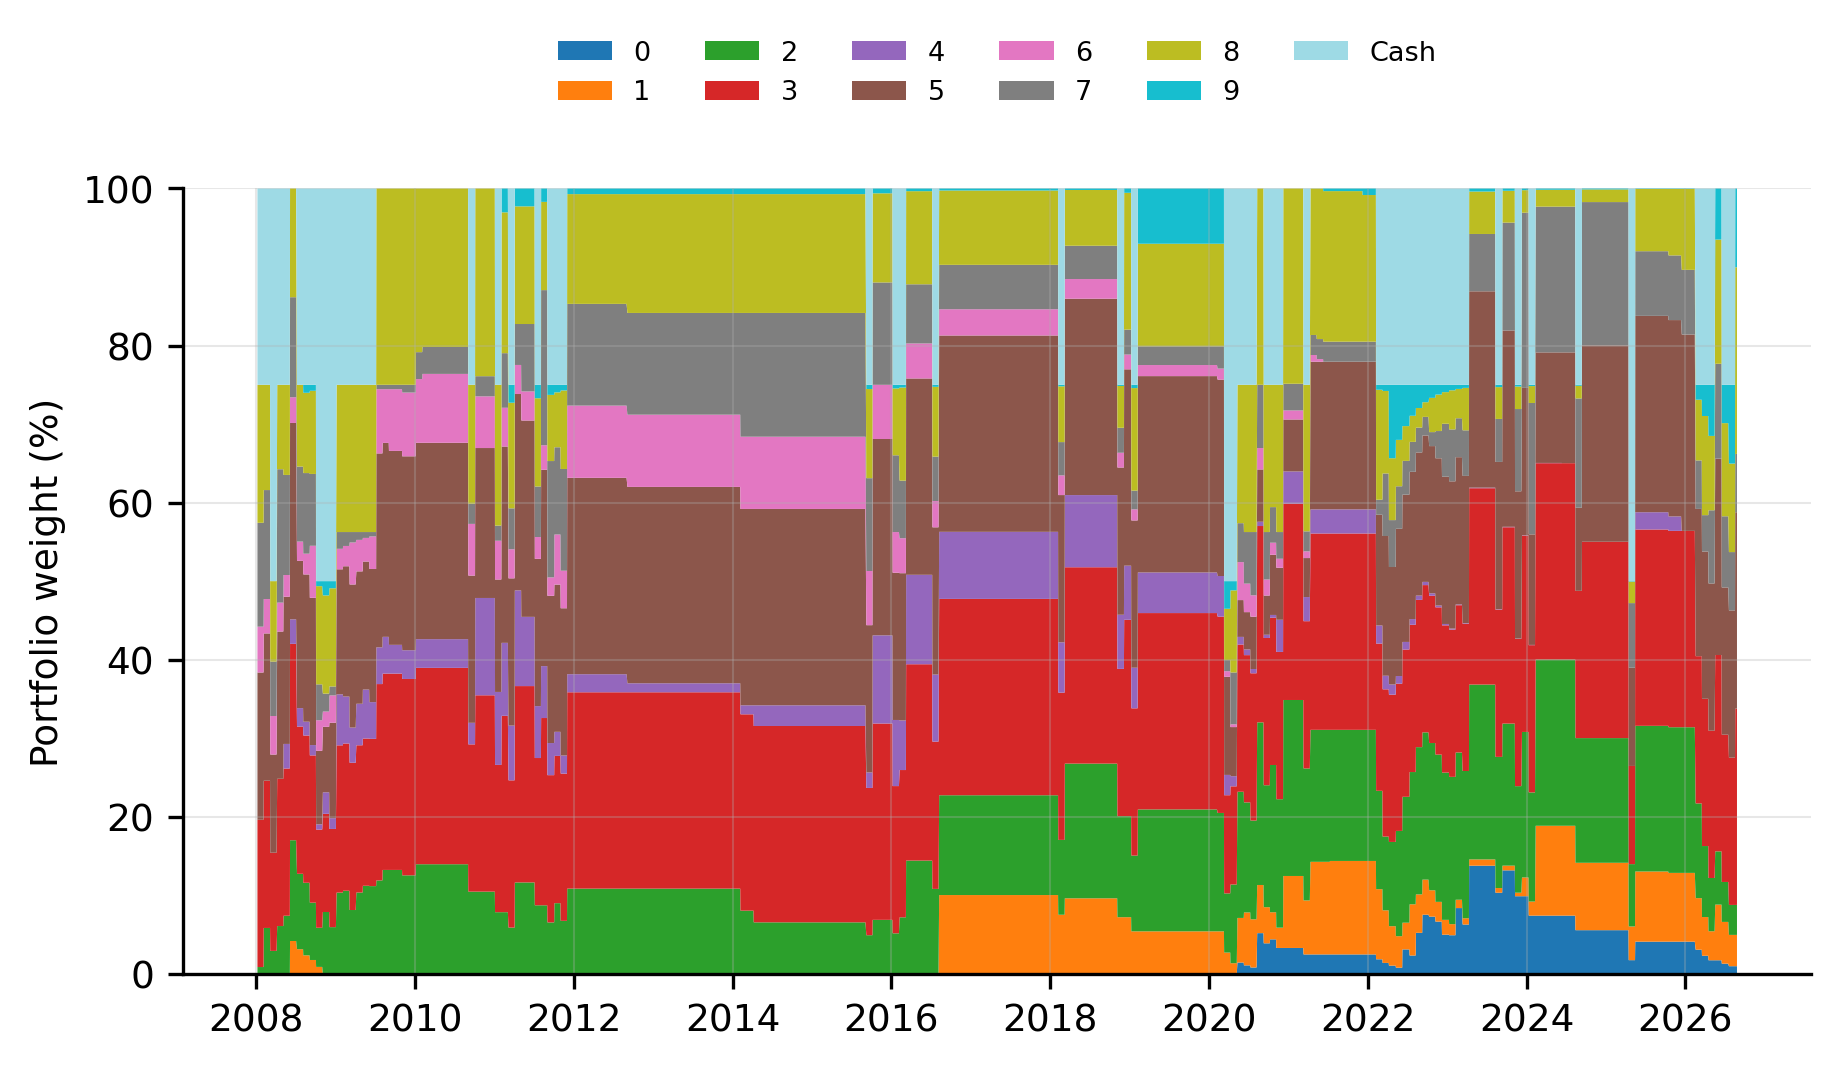
\includegraphics[width=\textwidth]{single column/images/fig_alloc.png}
\caption{Portfolio weights over time, including the cash residual}
\label{fig:alloc}
\end{figure*}

\begin{figure*}[t]
\centering
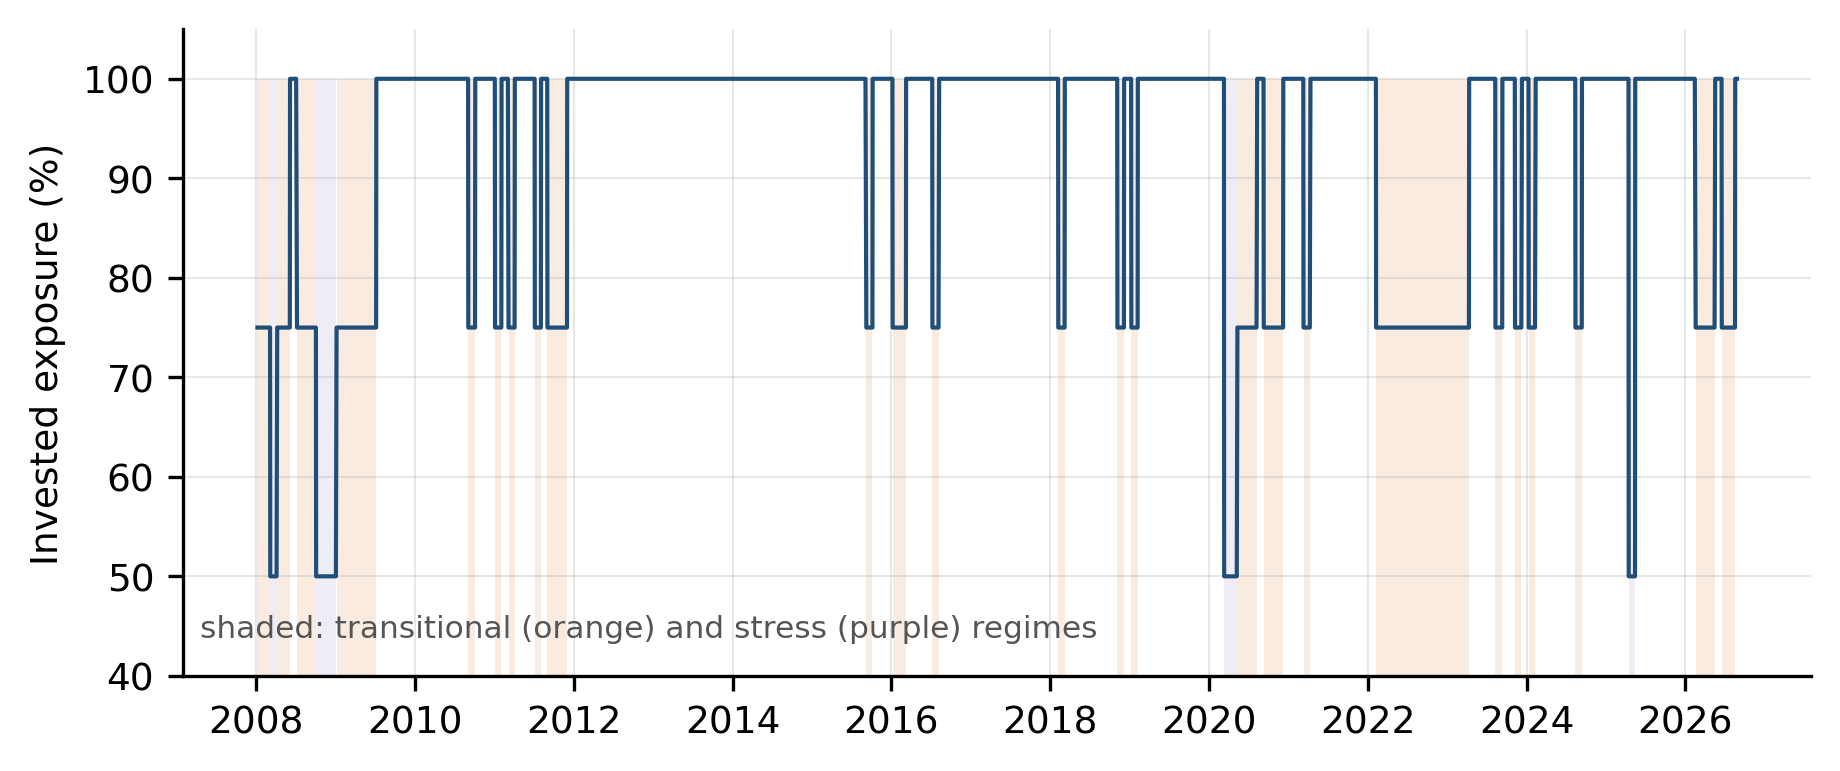
\includegraphics[width=\textwidth]{single column/images/fig_exposure.png}
\caption{Invested exposure over time, with transitional and stress regimes shaded}
\label{fig:exposure}
\end{figure*}

The allocation is diversified and stable. The largest position sits at the 25 per cent
cap on average, the effective number of assets averages 5.40 and never falls below
4.60, and annual one-way turnover is 0.96 times portfolio value, equivalent to
approximately 8.0 per cent of the portfolio traded at each monthly rebalance. Invested
exposure follows the regime, falling to a minimum of 50 per cent during the stress
state, which is the mechanism Figure~6 displays directly.

The cost sensitivity contains a result worth stating explicitly. Performance is not
monotone in the assumed cost: at zero assumed cost the Sharpe ratio is 0.773, below the
0.878 obtained at 10 basis points, even though no costs are deducted. The reason is
that the assumed cost enters the objective as a turnover penalty as well as entering
the return as a deduction. With the penalty removed, annual turnover rises from
0.96 to 4.04 times portfolio value as the optimiser chases small differences in the
estimated covariance matrix, and the resulting weight instability costs more than the
saved commissions are worth. The turnover penalty is therefore functioning as a
regulariser on the weight vector, and the framework is robust across the plausible cost
range of 5 to 25 basis points, over which the Sharpe ratio varies only between 0.846
and 0.893.

This section also resolves a defect in the framework as originally specified. In that
version the fused score entered the objective without the information-ratio scaling of
Equation~(\ref{eq:alpha}), so the linear term was expressed in the raw units of the
underlying indicators. On-balance volume takes values of order $10^{8}$ to $10^{9}$,
while annualised variances are of order $10^{-2}$. The linear term consequently
dominated the quadratic risk term by roughly ten orders of magnitude, the risk model
became irrelevant to the solution, and the optimiser returned a corner solution holding
a single asset on every rebalance date---an effective number of assets of exactly 1.00,
with one holding persisting for 1{,}364 of 1{,}421 sessions. The scaling in
Equation~(\ref{eq:alpha}) removes the defect by placing the linear term on a return
scale, and Table~\ref{tab:turnover} reports the corrected behaviour. The failure was one of units, not
of the optimiser or of the risk model.

\subsection{Regime Model Diagnostics}
\label{sec:regimefit}

Table~\ref{tab:regimefit} reports the mixture model's order selection statistics and the properties of
the three-state solution.

\begin{table}[!ht]
\centering
\caption{Regime model diagnostics. Order selection is computed on the full feature
history; state characteristics and the transition matrix come from the three-component
solution. Out-of-sample shares are the states actually assigned by the expanding-window
refits used in the backtest.}
\label{tab:regimefit}
\small
\begin{tabular}{p{3.2cm}rrrrr}
\hline
\multicolumn{6}{l}{\textit{Order selection}} \\
\hline
\textbf{Components} & 2 & 3 & 4 & 5 & 6 \\
AIC & 21944 & 20785 & 20571 & 20478 & 20372 \\
BIC & 22016 & 20896 & 20720 & 20667 & 20599 \\
\hline
\multicolumn{6}{l}{\textit{Three-state solution}} \\
\hline
& \textbf{Calm} & \textbf{Transitional} & \textbf{Stress} & & \\
Annualised volatility & 12.22\% & 20.04\% & 47.07\% & & \\
Annualised momentum & $+16.04$\% & $-1.25$\% & $-15.97$\% & & \\
Share of sessions, in sample & 63.6\% & 31.2\% & 5.2\% & & \\
Share of sessions, out of sample & 71.4\% & 25.5\% & 3.1\% & & \\
Mean run length (sessions) & 25.3 & 11.1 & 17.1 & & \\
Self-transition probability & 0.961 & 0.910 & 0.941 & & \\
\hline
\multicolumn{6}{l}{\textit{Realised performance within each out-of-sample state}} \\
\hline
& \textbf{Calm} & \textbf{Transitional} & \textbf{Stress} & & \\
Sessions & 3346 & 1196 & 147 & & \\
Strategy Sharpe & 1.144 & 0.196 & 1.039 & & \\
Equal-weight Sharpe & 0.916 & 0.561 & 0.356 & & \\
\hline
\end{tabular}
\end{table}

The order selection statistics are reported rather than used. Both AIC and BIC continue
to fall over the range examined, from 21944 and 22016 at two components to 20372 and
20599 at six, so neither criterion selects an interior optimum and neither supports the
choice of three components. This behaviour is expected: a mixture fitted to persistent,
heavy-tailed financial features will absorb tail observations into additional
components indefinitely, and the criteria reward it for doing so. The choice of three
is made instead on persistence and interpretability, and Table~\ref{tab:regimefit} supplies the grounds.
The three states are economically distinct---annualised volatility of 12.2, 20.0 and
47.1 per cent, with annualised momentum of $+16.0$, $-1.3$ and $-16.0$ per cent---and
they persist, with self-transition probabilities between 0.910 and 0.961 and mean run
lengths of 11 to 25 sessions. States of that duration can be acted upon at a monthly
rebalancing frequency. Finer partitions produce shorter-lived states that the
rebalancing schedule cannot exploit, and the transition matrix is close to
tridiagonal---the estimated probability of moving directly between the calm and the
stress state, in either direction, is zero---which indicates that the ordering recovered by
sorting components on volatility is economically meaningful rather than arbitrary.

The final panel shows where the framework's advantage arises. In the stress state the
framework attains a Sharpe ratio of 1.039 against 0.356 for the benchmark, and in the
calm state 1.144 against 0.916. It underperforms materially only in the transitional
state, 0.196 against 0.561, which is consistent with the 2021 result in Table~\ref{tab:years}: a
state that is genuinely ambiguous causes the risk budget to reduce exposure in
advances that turn out to continue. Figure~7 shows the identified states over time and
Figure~8 the behaviour of the two composites.

\begin{figure*}[t]
\centering
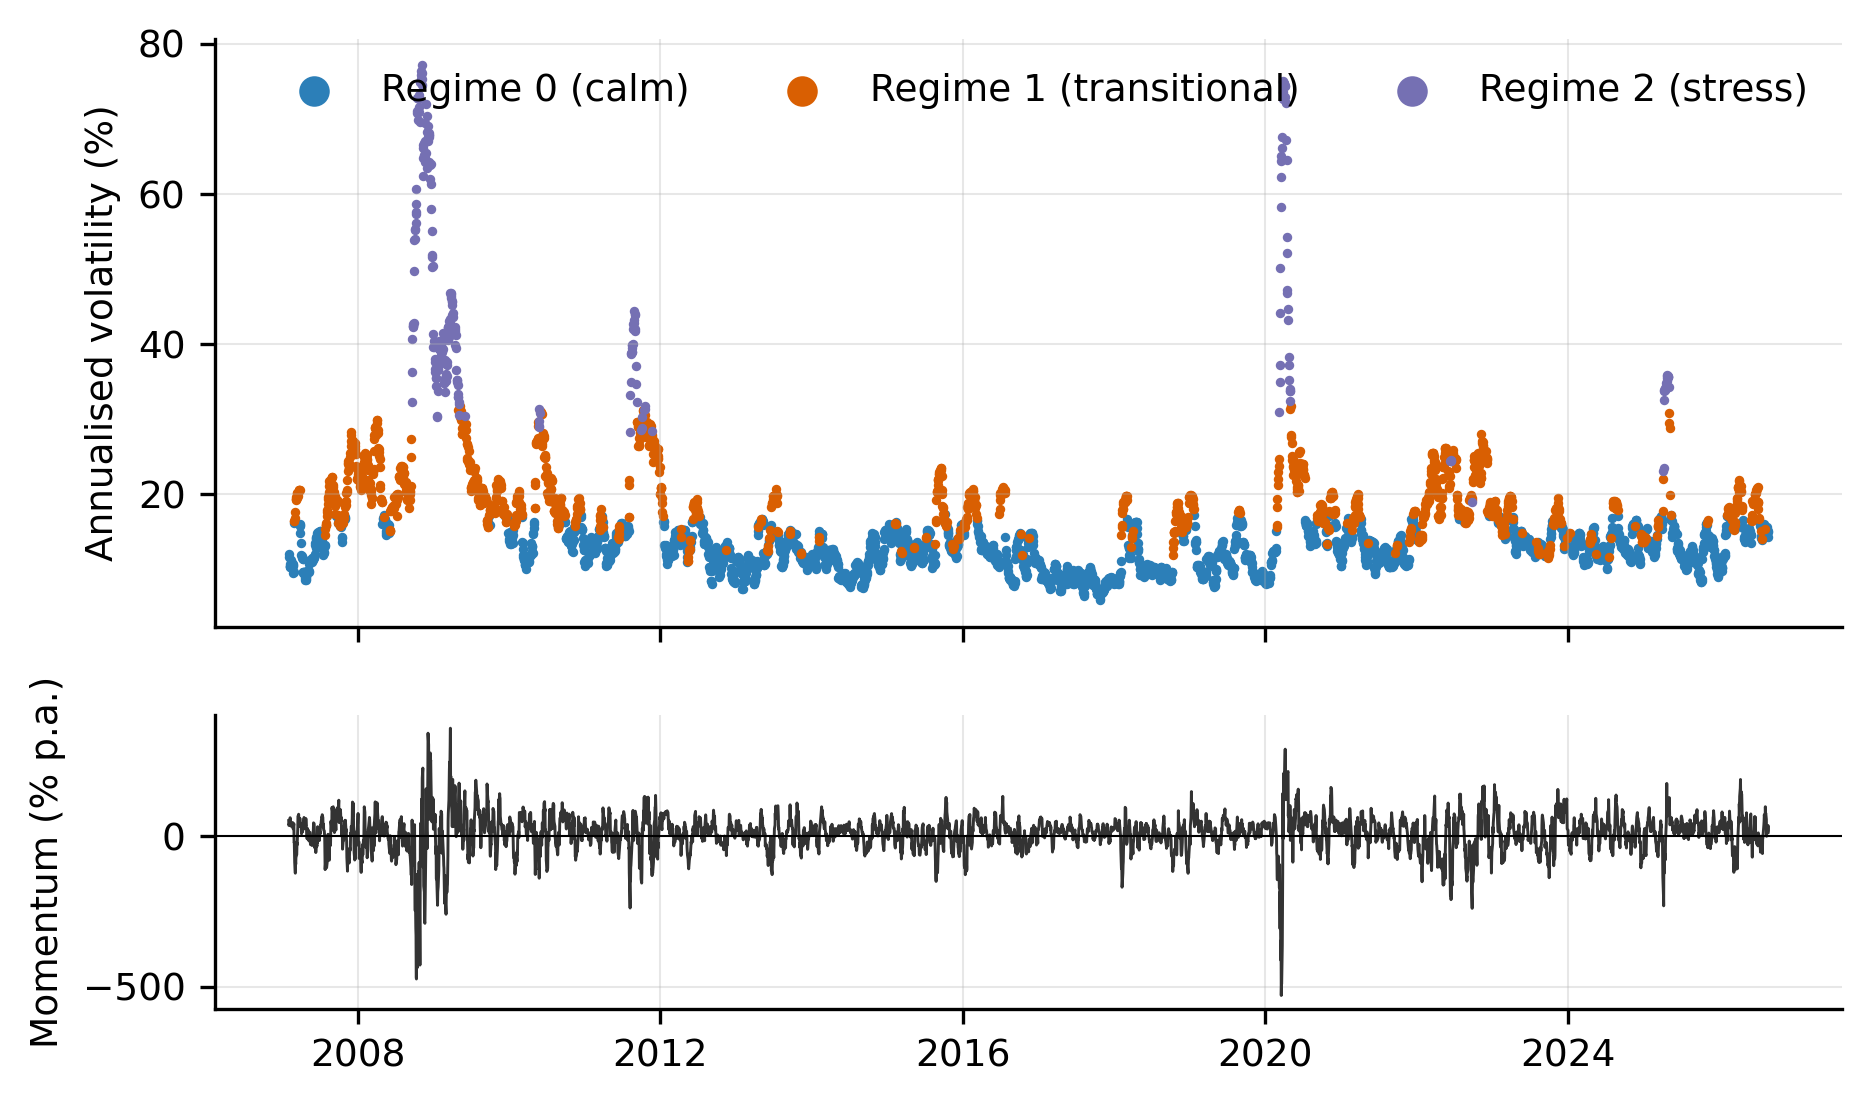
\includegraphics[width=\textwidth]{single column/images/fig_regimes.png}
\caption{Identified market states, with the underlying volatility and momentum features}
\label{fig:regimes}
\end{figure*}

\begin{figure*}[t]
\centering
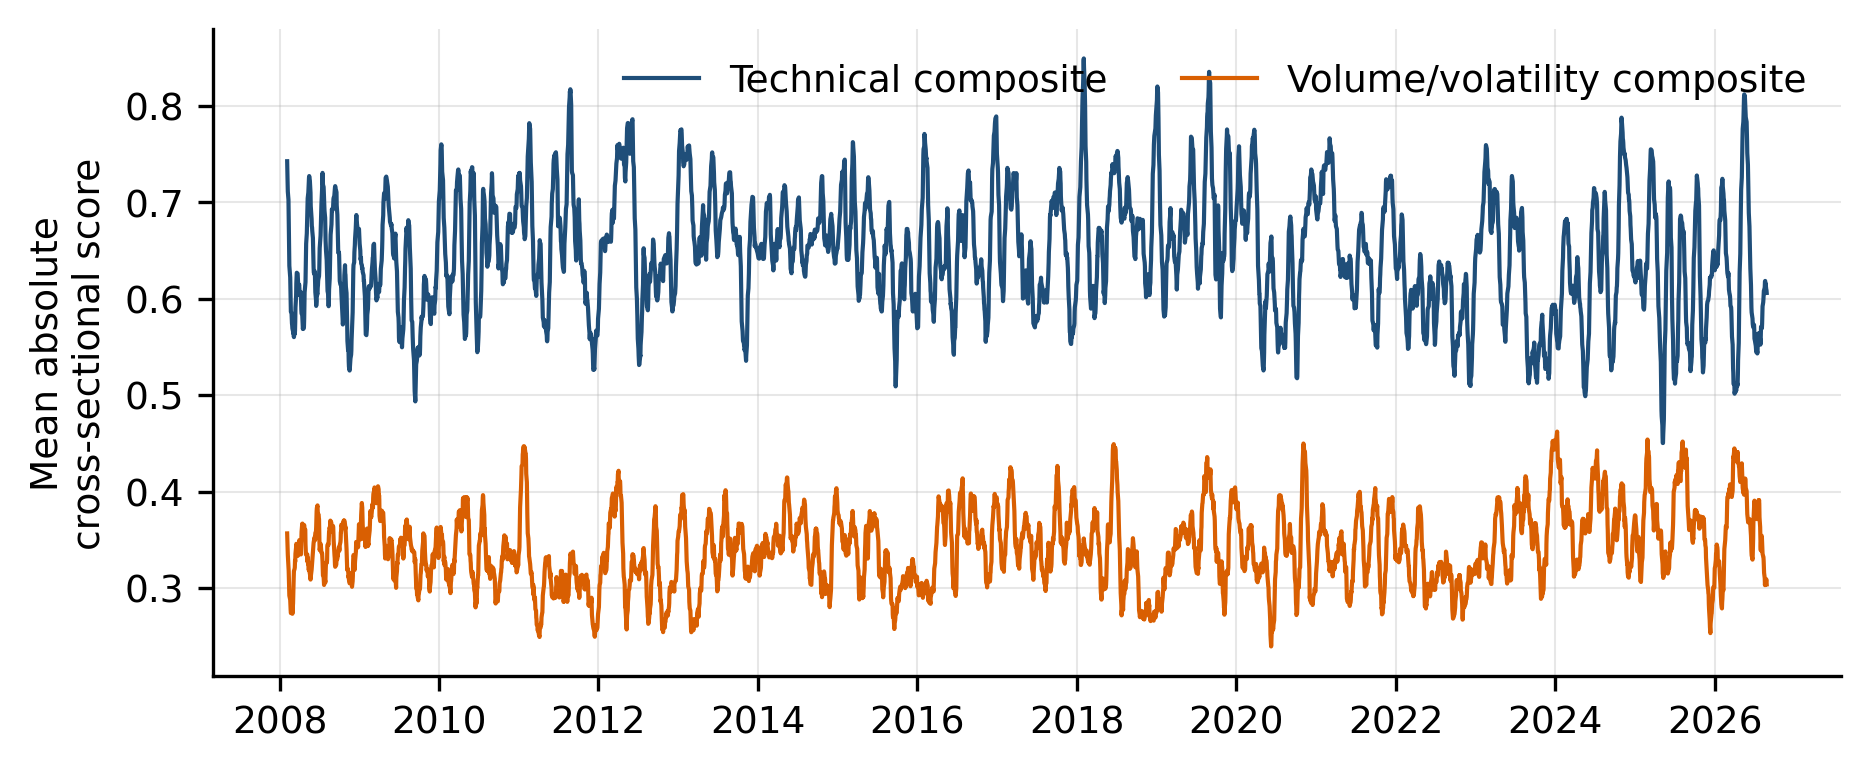
\includegraphics[width=\textwidth]{single column/images/fig_signal.png}
\caption{Mean absolute cross-sectional score of each composite, 21-session moving average}
\label{fig:signal}
\end{figure*}

\subsection{Statistical Significance}

Table~\ref{tab:inference} reports inference on the daily excess return series and on the Sharpe
difference.

\begin{table}[!ht]
\centering
\caption{Inference against the equal-weighted benchmark. Bootstrap intervals are from a
stationary block bootstrap with 21-session blocks and 2{,}000 replications.}
\label{tab:inference}
\small
\begin{tabular}{p{6.4cm}r}
\hline
Mean excess return over benchmark, annualised & $-3.31$\% \\
Paired $t$-statistic & $-1.369$ \\
$p$-value & 0.171 \\
Newey--West $t$-statistic, ten lags & $-1.699$ \\
\hline
Strategy Sharpe ratio, 95\% bootstrap interval & $[0.394, \; 1.368]$ \\
Benchmark Sharpe ratio, 95\% bootstrap interval & $[0.180, \; 1.165]$ \\
Sharpe difference, median & $+0.242$ \\
Sharpe difference, 95\% bootstrap interval & $[-0.102, \; 0.574]$ \\
Bootstrap probability that the difference is not positive & 0.088 \\
\hline
\end{tabular}
\end{table}

The results must be stated carefully. The framework's mean return is below the
benchmark's, and that shortfall is not statistically significant ($p = 0.171$). The
Sharpe difference of $+0.250$ has a bootstrap median of $+0.242$ and a 95 per cent
interval of $[-0.102, 0.574]$ that includes zero; the bootstrap probability that the
difference is not positive is 0.088. On an eighteen-year sample, therefore, the Sharpe
improvement is not significant at conventional levels, and the paper does not claim
that it is. Extending the sample by the 665 sessions of the holdout narrowed that
interval---its lower bound moves from $-0.194$ on the pre-2024 data to $-0.102$---without
crossing zero, which is the expected behaviour of a real but modest effect measured on
a sample that remains too short.

What is robust is not the point estimate but its consistency. The Sharpe advantage
appears in 18 of 18 specifications, the drawdown advantage in 18 of 18 and in 18 of 19
calendar years, and the outperformance in all four stress episodes. Eighteen years of
daily data contain few independent observations of the events that matter for a
drawdown claim---four, on the evidence of Table~\ref{tab:episodes}---and no amount of daily
sampling converts that into statistical power. The appropriate conclusion is that the
drawdown reduction is consistent and mechanically explicable, and that the Sharpe
improvement, while positive under every specification examined, is not established at
conventional significance.

\subsection{Secondary Universe: Mega-Capitalisation Equities}
\label{sec:megacap}

The framework was also run without modification on the ten mega-capitalisation US
equities of the original study, over the same 2018--2026 download window, giving 1{,}920
evaluated sessions from January 2019. Table~\ref{tab:megacap} reports the outcome, which
is unfavourable on risk-adjusted return.

\begin{table}[!ht]
\centering
\caption{Secondary universe: ten mega-capitalisation US equities, 2019--2026}
\label{tab:megacap}
\small
\begin{tabular}{p{4.8cm}rrrr}
\hline
& \textbf{CAGR} & \textbf{Volatility} & \textbf{Sharpe} & \textbf{Max DD} \\
\hline
Regime-conditional strategy & 17.02\% & 14.87\% & 1.145 & $-20.45$\% \\
Equal-weight benchmark & 33.52\% & 24.45\% & 1.371 & $-33.63$\% \\
Equal-weight at strategy volatility & 20.08\% & 14.87\% & 1.350 & $-21.41$\% \\
No regime timing, same average exposure & 18.82\% & 16.82\% & 1.119 & $-30.36$\% \\
\hline
\end{tabular}
\end{table}

The framework loses on risk-adjusted return, 1.145 against 1.371, and gives up 15.09
percentage points of annual return, a shortfall that is statistically significant
($t = -2.791$, $p = 0.005$). Its defensive behaviour nevertheless survives intact:
maximum drawdown improves from $-33.63$ to $-20.45$ per cent, it wins on drawdown in
8 of 8 calendar years while winning on Sharpe ratio in only 3, and it outperforms in
both stress episodes this window contains, by 12.50 percentage points during the 2020
crash and 12.60 percentage points during the 2022 bear market.

The regime layer itself continues to behave as the primary results describe. Against the
matched-exposure control it improves the Sharpe ratio slightly, 1.145 against 1.119, and
improves maximum drawdown substantially, from $-30.36$ to $-20.45$ per cent. The
risk-timing effect identified in Section~\ref{sec:ablation} therefore reproduces in a
universe on which the framework loses overall, which is the relevant test of whether that
effect is specific to the primary sample. What fails here is not the regime layer but the
decision to hold the resulting portfolio in place of the benchmark.

The reason is a property of the universe rather than of the framework. Ten
mega-capitalisation US equities are close to a single factor bet: correlations are high,
there is no low-volatility asset to rotate into, and the risky sleeve therefore carries
roughly 15 per cent annualised volatility against 6 per cent in the multi-asset case.
De-risking in such a universe can only move capital to cash, so the framework
systematically forgoes return during an exceptional advance and recovers only part of it
in drawdowns. This bounds the applicability of the framework directly: it requires a
universe with genuine dispersion in asset volatility, and it should not be expected to
add value in a concentrated, single-sector one. The originally submitted version of this
study used exactly such a universe, which is why its results are superseded here.
